\documentclass[a4paper,12pt,titlepage]{article}
\usepackage[T1]{fontenc}
\usepackage[brazil]{babel}
\usepackage[utf8x]{inputenc}
\usepackage{graphicx}
\usepackage{times}
\usepackage{ucs}
\usepackage{url}



\title{Trabalho de conclusão de curso \\
BOINC + R: Executando rotinas de bioinformática em grades oportunistas} 


\author{Aluno: Rodrigo L. M. Flores \and
        Orientador: Roberto Hirata Jr. }


\date{\today}

\begin{document}

\maketitle

\nocite{wiki:volunteercomputing}
\nocite{wiki:interpretedlanguage}
\nocite{wiki:boinc}
\nocite{wiki:r}
\nocite{boinc_wrapper}
\nocite{hungaro}
\nocite{nytimes}

\tableofcontents

\pagebreak

\part{Parte objetiva}

\section{Introdução}


O foco deste projeto é atrair a atenção dos alunos do IME em relação a disciplina de física ministrada no curso de bacharelado em ciência da computação.
Com o simulador podemos integrar melhor os alunos aos assuntos abordados na física com demonstrações de ambientes físicos, 
integrando exercícios programas (EP) e também para ser utilizado em sala de aula.

\subsection{Física na computação}

A disciplina de Física (FAP-0126), oferecida no curso de BCC, é puramente teórica e não mostra nenhuma relação com a Ciência da Computação. Isso torna a disciplina menos interessante e frequentemente faz os alunos pensarem: "Para que serve esta disciplina?".
Para motivar os alunos e ilustrar melhor a relação entre as disciplinas básicas (Física, Estatística, Álgebra e Cálculo) com a Ciência da Computação, pretendemos criar uma biblioteca gráfica de simulação. Esta biblioteca será capaz de realizar uma leitura de dados de uma simulação de um EP e mostrar graficamente o resultado da simulação, por exemplo.
Esta biblioteca também proporcionará um ambiente de simulação específico e pronto para ser mostrado em salas de aula.
\subsection{Integração com a computação}

Existem muitos problemas ao tentar simular um ambiente físico com a computação. Temos o problema do tempo de simulação, 
que é o tempo que damos para os objetos físicos se interagirem e tomar o rumo necessário para refletir a realidade.
Existem alguns conceitos como broad phase, que é a fase em que os objetos são filtrados para realizarmos depois a narrow phase que é onde verificamos se aconteceu 
alguma colisão entre os objetos.

\subsection{Simulador}

A idéia do simulador é poder mostrar os problemas que encontramos ao tentar simular um ambiente físico com montagem de demonstrações. 


\newpage

\section{Conceitos e tecnologias utilizadas}

O desenvolvimento do projeto incluiu diversas tecnologias, sendo as principais a linguagem de Programação \emph{R} e o middleware
para computação voluntária \emph{BOINC}. Dentre os conceitos estudados, podemos destacar a computação em grade.  

\subsection{BOINC}

O BOINC, cujo nome é uma sigla para \textit{Berkeley Open Infrastructure for Network Computing}, é um middleware 
para computação em grade e voluntária e foi criado na Universidade de Berkeley, Califórnia, Estados Unidos.

Inicialmente, o projeto consistia em gerenciar o projeto \textit{SETI@HOME} que possuía dois objetivos:

\begin{itemize}
	\item Provar a viabilidade e a praticidade do conceito ``computação em grade distribuída'';
	\item Fazer um trabalho científico útil: uma análise observacional para detectar vida inteligente fora da Terra.
\end{itemize}

O primeiro objetivo foi concluído com sucesso e o resultado é o \textit{BOINC}. O segundo falhou: nenhuma evidência de 
vida inteligente fora da Terra foi encontrada até hoje. 

Dentre os diversos motivos para a utilização do \emph{BOINC}, baseados no artigo \cite{boinc}, podemos destacar:

\begin{itemize}
  \item \textbf{Mais utilizado -} Quando comparado com outros \emph{middlewares} semelhantes como o \textit{middleware} 
\emph{Condor} ou o \emph{Xtremweb}, o \emph{BOINC} é mais utilizado e há pacotes para o \emph{BOINC} nas 
distribuições \emph{Linux} mais populares;
  \item \textbf{Amplamente utilizado -} O \emph{BOINC} é utilizado em diversas áreas como previsão do tempo, física,
astrofísica, biologia, entre outras;
  \item \textbf{Suporte da comunidade -} Baseado no espírito de ajuda mútua existente em comunidades de software livre, é 
possível ter dúvidas esclarecidas quanto ao funcionamento do \emph{BOINC} de maneira fácil e desburocratizada. Por ser um projeto
cujas listas de discussão e canais de \textit{chat} são movimentados é bem comum alguns problemas serem resolvidos em questão de 
poucos dias;
  \item \textbf{Estrutura simples -} O BOINC possui uma estrutura simples de comunicação: um servidor que armazena e 
distribui os trabalhos a serem feitos e os clientes que tem o papel de processar os trabalhos;
  \item \textbf{Documentação completa -} A página oficial do BOINC possui muita do\-cu\-men\-ta\-ção e muitos tutoriais explicando
cada detalhe da instalação e configuração de um projeto. Há também páginas não oficiais, como o Wiki não oficial do \emph{BOINC}\footnote{cujo endereço é \url{http://www.boinc-wiki.info}},
que também servem de ajuda.
\end{itemize}



\subsubsection{Funcionamento do BOINC}


Cada unidade de processamento no BOINC é chamada de \emph{workunit} e é constítuida de arquivos executáveis e 
arquivos de entrada. Depois de processado, os arquivos de saída gerados são enviados para o servidor que
normalmente armazena estas saídas em um banco de dados ou em um arquivo.

Para gerar um workunit são necessários dois arquivos XML, um deles de\-ta\-lhan\-do a entrada e o 
outro detalhando a saída. Para facilitar a escrita do programa, precisamos escrever para cada arquivo um nome lógico 
que ao enviar e receber o cliente renomeia o arquivo. Por exemplo, temos um programa que lê um arquivo chamado 
\verb#input# e escreve no arquivo \verb#output#, para podermos ter muitos arquivos de entrada com nomes diferentes, quando
criamos uma \emph{workunit}, o servidor coloca um nome único e semelhante ao da workunit nos arquivos de entrada e saída que serão renomeados
pelo cliente para o nome lógico.

O processamento é realizado pelo cliente: o arquivo binário é executado e enquanto ele é executado há um checkpoint
que permite em caso de interrupções retomar o processamento de um determinado ponto. Finalizado o processamento, 
na próxima atualização o cliente avisará ao servidor que o processamento foi finalizado. Um diagrama do funcionamento pode
ser visto na figura \ref{funcionamento-boinc}. 


\begin{figure}[!h]
  \centering
  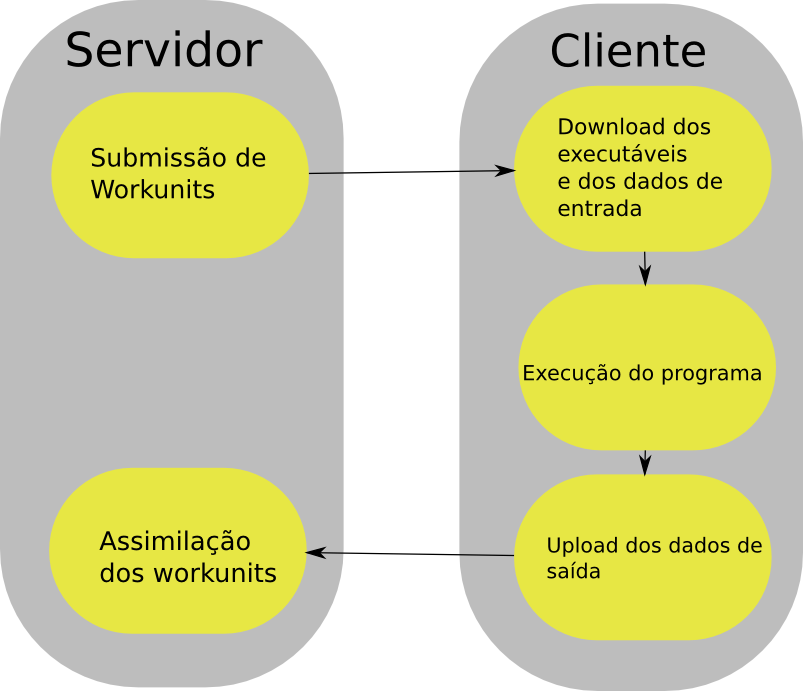
\includegraphics[scale=0.5]{boinc-schema.png}
  \caption{Funcionamento do BOINC}
  \label{funcionamento-boinc}
\end{figure}

\newpage

\subsubsection{Wrapper}


O \emph{Wrapper} é um programa escrito utilizando a \emph{API} do \emph{BOINC}, cujo objetivo é executar aplicações legadas, 
i.e. aplicações que não utilizam a API do \emph{BOINC}, utilizando o \textit{BOINC}. Há uma versão do Wrapper distribuída junto com o 
\textit{BOINC} que utiliza um arquivo XML, mas existe uma outra opção descrita no artigo \cite{hungaro} que utiliza um shell para a 
execução dos aplicativos. Os diagramas de funcionamento do 
\emph{BOINC} com um programa escrito com a API e com o wrapper podem ser vistas nas figuras \ref{boinc-api} e \ref{boinc-wrap} 
respectivamente.


O arquivo XML de execução tem a seguinte estrutura:

\begin{verbatim}
<job_desc>
    <task>
        <application>foobar</application>
        [ <stdin_filename>stdin_file</stdin_filename> ]
        [ <stdout_filename>stdout_file</stdout_filename> ]
        [ <stderr_filename>stderr_file</stderr_filename> ]
        [ <command_line>--foo bar</command_line> ]
    </task>
    [ ... ]
</job_desc>
\end{verbatim}

Neste XML, o único campo obrigatório é o \emph{application}, que é a aplicação
que será executada e pode ser distribuída junto com a aplicação ou já existir no 
computador que o cliente estará instalado (para este segundo caso é necessário
informar o caminho inteiro do executável). É possível ter mais de uma tag
task, e o wrapper as executará sequencialmente. É de responsabilidade
do \textit{Wrapper} perceber se a execução do programa foi feita com sucesso, 
mas não é responsabilidade dele verificar se os pré-requisitos que o programa necessita
estão presentes no sistema (se isso por ventura acontecer, o arquivo de saída não aparecerá 
no servidor, porém a execução será dada como correta no banco de dados). 


\begin{figure}[!h]
  \centering
  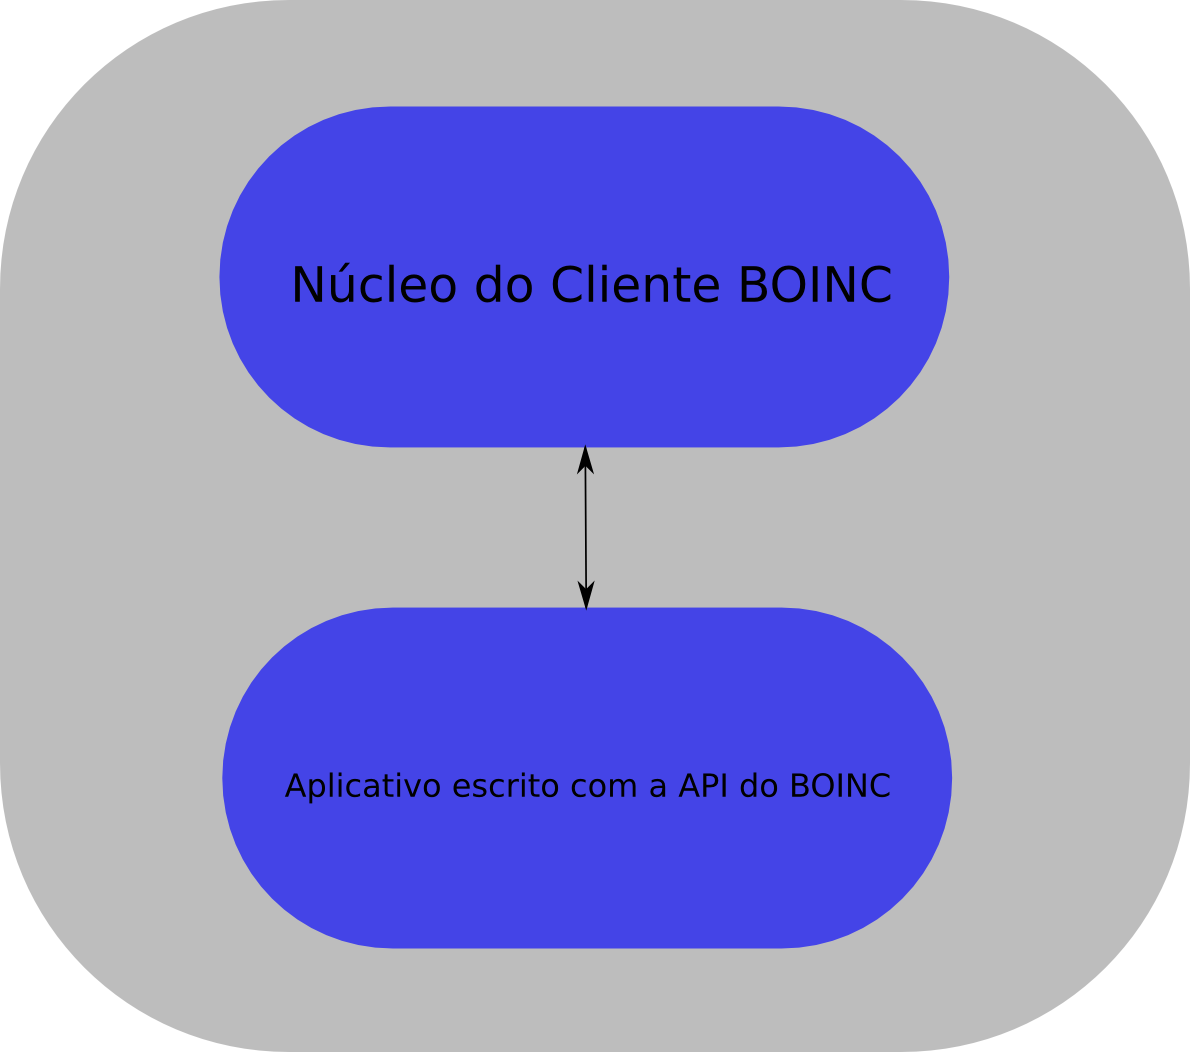
\includegraphics[scale=0.3]{boinc-api.png}
  \caption{Funcionamento do BOINC utilizando uma aplicação que utiliza sua API}
  \label{boinc-api}
\end{figure}


\begin{figure}[!h]
  \centering
  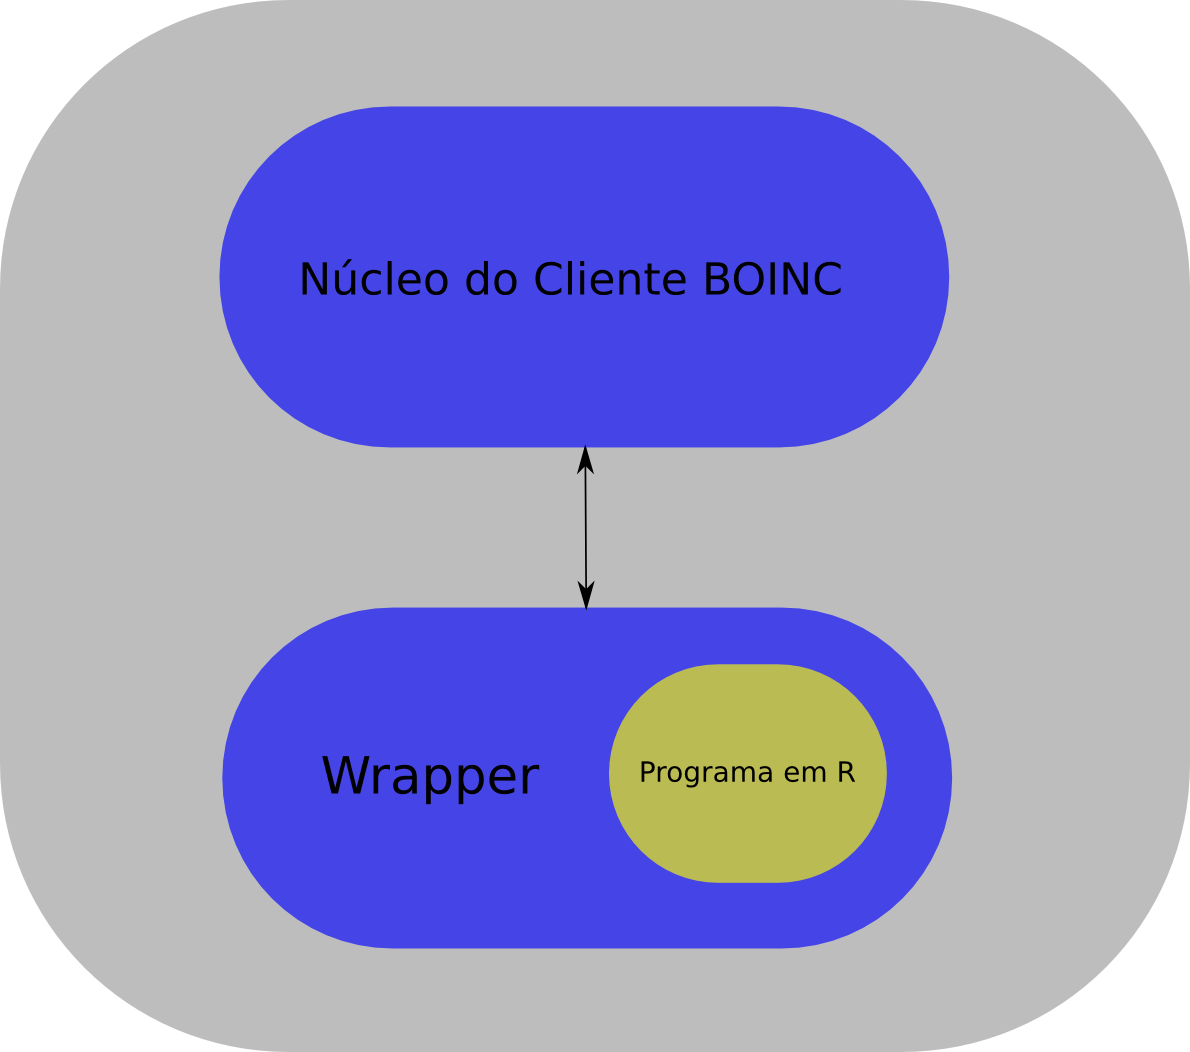
\includegraphics[scale=0.3]{boinc-wrap.png}
  \caption{Funcionamento do BOINC utilizando uma aplicação que utiliza o \emph{wrapper}}
  \label{boinc-wrap}
\end{figure}


\subsection{R}

A linguagem de programação estatística \emph{R} é uma implementação da linguagem \emph{S} e foi criada por Ross Ihaka e Robert
Gentleman na Universidade de Auckland, da Nova Zelândia. A linguagem e ambiente para cálculos estatísticos é considerada
padrão \cite{nytimes} %http://www.nytimes.com/2009/01/07/technology/business-computing/07program.html?_r=1
na área de análise de dados e além do ambiente acadêmico, empresas como \emph{Google}, \emph{Pfizer} e \emph{Merck} a utilizam em seus
processos de mineração de dados. 

Dentre as facilidades que seu uso proporciona, podemos citar as seguintes:

\begin{itemize}
  \item Grande quantidade de funções estatísticas de uso cotidiano na análise de dados
como cálculo de média, desvio padrão, ajuste de curvas, análise de séries temporais. Há também funções mais complexas como por 
exemplo implementações de algoritmos de \emph{clustering}. 
  \item Utilizando o \emph{R} é possível fazer operações em tabelas semelhantes a que normalmente 
são feitas em bancos de dados relacionais como seleção de linhas em tabelas que atendem
certas condições. 
  \item O \emph{R} possui também rotinas de manipulação de matrizes e resolução de sistemas lineares, que são essenciais
em qualquer tarefa de cálculo numérico. 
  \item Gráficos de alta qualidade dos mais variados tipos e para os mais variados propósitos com uma qualidade alta 
também podem ser feitos com o \emph{R}. 
  \item A facilidade de se criar e de se obter pacotes, que nada mais são que conjuntos de rotinas agrupadas, é outro fator
importante: é muito simples criar pacotes e documentá-los. Para disponibilizá-los, pode se submeter um pedido de aprovação 
de para disponibilização no repositório oficial (\url{http://cran-r.c3sl.ufpr.br/})  
do \emph{R}, que possui $2076$ pacotes para os mais diversos fins. O repositório possui \emph{mirrors} espalhados por
todo o mundo, inclusive no Brasil.  
\end{itemize}

Além destes motivos, o artigo \cite{bioconductor} dispõe outros motivos para a utilização do \emph{R} e de seu
pacote para análise de dados de de bioinformática \emph{Bioconductor}.

\begin{itemize}
  \item \textbf{Transparência -} Muitas metodologias de análise na área de biologia e bioinformática computacional
são extremamente complexas e muitas etapas são necessárias na conversão de informação bruta (como por exemplo imagens 
escaneadas de \emph{microarray}). Não se sabe a priori, como as análises podem ser sensíveis a estes fatores, e portanto
trabalhos referenciados na área normalmente expõe todo o processo. O uso de mesmo ambiente e das mesmas ferramentas 
facilita bastante esta transparência;
  \item \textbf{Reprodutibilidade -} Experimentos na área de biologia molecular devem publicar listas de ingredientes
e algoritmos para criar substâncias e processos. Um resultado só pode ser verificado se existir uma obediência a 
um protocolo. Seguindo esta linha, a mineração de dados também deve ser bem descrita e tanto o código fonte 
como os dados nos quais a análise é baseada são normalmente publicados junto com um trabalho nesta área. Utilizar
um mesmo ambiente, que pode ser obtido gratuitamente, para qualquer plataforma, com pacotes 
facilmente extensíveis também facilita este processo.
  \item \textbf{Eficiência do desenvolvimento -} Se o pacote foi por ventura desenvolvido para alguma necessidade, ele pode ser publicado
, melhorado, estudado por outros cientistas, e pode ter seu leque de funcionalidades aumentado caso seu uso siga padrões
de código aberto. Para isso é necessário que esteja bem documentado. Tanto o \emph{R} como o \emph{Bioconductor} são softwares
de código aberto e desfrutam desta qualidade.
  \item \textbf{Prototipagem -} Como o \emph{R} é uma linguagem em um nível mais alto que ou\-tras linguagens como \emph{C} ou
\emph{FORTRAN}, programar novas rotinas é bem mais simples. Mesmo não tendo uma execução tão eficiente como em outras
linguagens, pode ser utilizado como protótipo, para depois ser implementado em uma linguagem mais eficiente. 

\end{itemize}

\subsection{Utilização do \emph{BOINC} para o processamento de rotinas na linguagem \emph{R}}

Dentre as possibilidades de processamento em grade para a linguagem \emph{R}, es\-co\-lhe\-mos o \emph{BOINC} para o processamento em grade.
Dentre os motivos, podemos citar:

\begin{itemize}
  \item \textbf{Código aberto -} Ambas as tecnologias são de código aberto e possuem licenças que permitem a utilização das duas
ferramentas para qualquer propósito, além da obtenção gratuita e da possibilidade de estudo do código fonte das duas tecnologias.
Outro ponto forte em comum entre elas é a presença de uma comunidade ativa, com fóruns, listas de discussão e canais de IRC;
  \item \textbf{Multiplataforma -}  Em redes de universidades e empresas é muito comum a utilização de sistemas tanto 
\emph{Linux} como \emph{Windows}. Em ambientes nos quais há muito desenvolvimento de programas, o \emph{Linux} acaba
sendo bastante utilizado, já para um usuário cotidiano o Windows acaba sendo a opção mais comum. Ter uma solução
que utilize tanto computadores com sistemas \emph{Linux} como computadores com sistemas \emph{Windows} é essencial 
para sua utilização. Como o \emph{R} e o \emph{BOINC} já tem versões para estes dois sistemas, assim como o \emph{wrapper}, 
fica então possível a utilização multiplataforma da grade. Lembrando que a utilização multiplataforma deve funcionar para um mesmo
projeto e sem distinção de workunits, de modo a ser indiferente à quem submete a utilização de qual sistema para a computação.
  \item \textbf{Execução inalterada de aplicações escritas em \emph{R} -} Utilizando o \emph{wrapper} é possível executar,
sem precisar alterar um byte do código, programas compilados. Utilizando como programa compilado o interpretador do 
\emph{R}, podemos executar rotinas do \emph{R} utilizando o \emph{wrapper}. Isso poupa o trabalho de reescrever
códigos já previamente escritos e em funcionamento;
  \item \textbf{Possibilidade de se utilizar pacotes do \emph{R} -} Como o \emph{R} possui uma notável extensibilidade com mais
de $2000$ pacotes, é de se esperar que um ambiente para executar rotinas nesta linguagem também seja capaz de automaticamente instalar
pacotes do \emph{R}, caso isto seja necessário. Utilizando o \emph{BOINC} e o \emph{wrapper} é possível utilizar estes pacotes,
sendo apenas necessário verificar se eles estão instalados e colocar no programa o comando de instalação caso não estejam.
\end{itemize}



\newpage

\section{Atividades realizadas}

Criamos algumas demonstrações básicas demonstrando a capacidade da plataforma Chipmunk e etc...

\subsection{Demonstrações}

falar sobre as demonstrações feitas.. Aqui tem que ficar bonito pq vamos colocar imagem

\subsection{Simulador}

falar sobre o que o simulador faz... 


\newpage

\section{Resultados e produtos obtidos}


O principal resultado deste trabalho foi fazer o \emph{Boinc} funcionar com rotinas em \emph{R}, tanto
nos ambientes \emph{Linux} como no ambiente \emph{Windows} % colocar marca registrada

\subsection{Implementação}

\subsubsection{Sistema Linux}

Para o ambiente \emph{Linux}, o processo foi relativamente simples: dado um arquivo com rotinas
do \emph{R} a serem executadas, é somente necessário alterar a permissão do arquivo para executável 
(via \verb#chmod +x arquivo.R#) e adicionar a seguinte linha no início do arquivo:

\begin{verbatim}
#!/usr/bin/Rscript
\end{verbatim}

Isso faz um sistema \emph{Linux} chamar o interpretador \emph{Rscript} para interpretar o arquivo  
e assim fazer a interpretação do arquivo. Esta solução permite não só que rotinas em \emph{R} sejam
executadas, mas sim qualquer script que tenha seu interpretador descrito na primeira linha.

A esta solução, demos o nome de \emph{Truque do Shebang}, pelos caracteres \verb'#!' serem chamados
popularmente de \emph{shebang}. Esta implementação foi relativamente simples: o BOINC possuía um tutorial
para executarmos programas compilados na grade e só o truque do shebang foi necessário.

Porém, para termos a mesma solução em ambos os sistemas, utilizamos a solução para 
Windows no sistema Linux. 

\subsubsection{Sistema Windows} %Marca registrada

Como o sistema Windows não permite utilizar script utilizando o \emph{shebang}, foi necessário 
utilizar um programa compilado escrito na linguagem C, que chamamos de \emph{Runner}, 
que usando a função \verb#system#, chama o interpretador com o arquivo.R como parâmetro. 

Esta solução permite inclusive que usemos scripts diferentes de R a cada vez que criamos um 
\emph{workunit}, assim como adicionar arquivos extra que por ventura fossem necessários para
o processamento. Esta maneira também funciona no \emph{Linux}, só que o \emph{Runner} precisa
ser compilado para o \emph{Linux} com o caminho para o interpretador correto. O programa também não faz
uma verificação para perceber se o \emph{R} está instalado, dando um resultado de conclusão positiva
no banco, mas sem arquivos de saída. 

A utilização do \emph{Runner} foi necessária devido ao \emph{Wrapper} não perceber corretamente
que o interpretador foi executado sem erros e, mesmo em execuções sem erros, o \emph{wrapper} 
recebia um valor de retorno do interpretador diferente de zero, o que ele percebia como um erro
e marcava o \emph{workunit} como inválido. Um diagrama exemplificando esse funcionamento pode ser visto 
na figura \ref{diagrama-boinc-wrapper-windows}. Para a execução ficar multiplataforma, foi necessário 
fazer uma pequena alteração no \emph{wrapper} na versão para \emph{Linux} modificando o nome do
arquivo XML do wrapper, já que em ambos os sistemas é necessária a utilização de um arquivo XML próprio.


A implementação no Windows foi bastante difícil: existem muitos pequenos detalhes que acabam
atrapalhando um pouco. Um dos exemplos foi especificar o caminho do executável: para o Windows acessar
um diretório específico devemos ``truncar'' os nomes de diretórios maiores que $8$ caracteres, sendo 
assim apontamos o caminho, trocando o oitavo e nono caractere do diretório por \verb#~1# 
e desprezando os seguintes. 
Alguns outros problemas foram relacionados à falta de mensagens de erro do BOINC mais amigáveis e
à falta de verificação das entradas: um \verb#XML# mal formatado causou um erro  no processamento
do workunit, quando isso deveria ser acusado na submissão do workunit. Outro problema foi um \emph{Bug}
nas configurações de compilação do \emph{wrapper} no Microsoft Visual Studio Express % Verificar 
que fazia referência a bibliotecas desnecessárias e inexistentes para a compilação do \emph{wrapper}
e isso só foi resolvido pelos desenvolvedores do \emph{BOINC} algumas semanas depois. 


\begin{figure}[!h]
  \centering
  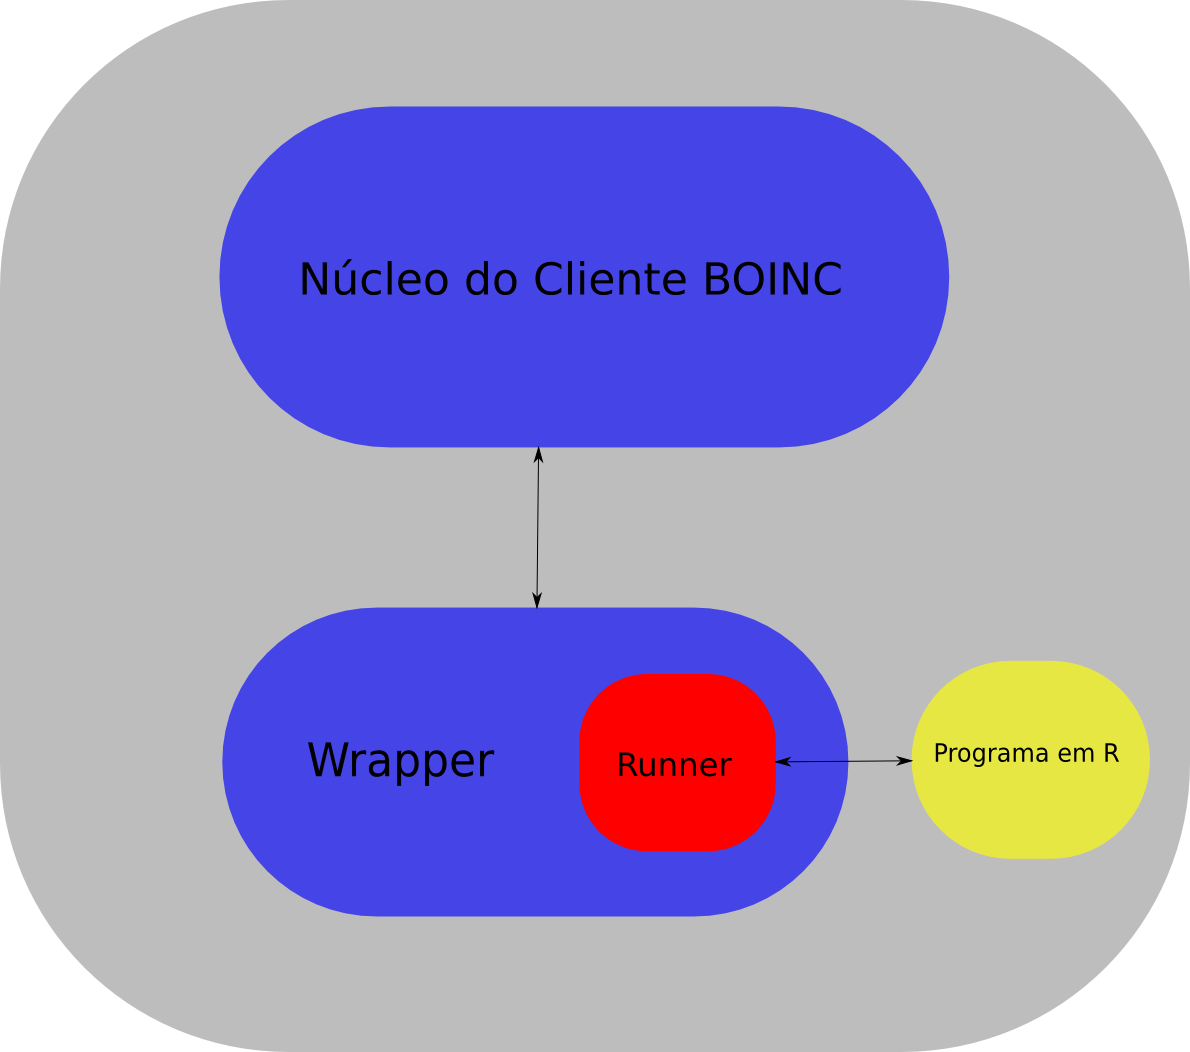
\includegraphics[scale=0.3]{boinc-diagram-runner.png}
  \caption{Diagrama do funcionamento do \emph{BOINC} com o \emph{Runner} e \emph{Wrapper}}
  \label{diagrama-boinc-wrapper-windows}
\end{figure}
 

\subsection{Discussão}



\subsubsection{Vantagens} 

As principais vantagens no uso do \emph{Boinc} para o processamento em grade são:

\begin{itemize}
  \item \textbf{Facilidade de se adicionar novos nós} - A instalação do BOINC em ambos os sistemas Linux e Windows é simples
e fácil de ser feita e nenhuma ação no servidor é necessária a cada instalação de nós. Além disso, é muito simples fazer
a replicação de configurações, tanto para o processamento, quanto para a conexão com o servidor para os computadores;
  \item \textbf{Processamento multiplataforma} - Para a grade funcionar na plataforma só são necessárias duas coisas: 
que o BOINC e o \emph{R} estejam disponível para a plataforma. As plataformas mais comuns 
(Linux $32$ e $64$ bits e Microsoft Windows) têm ambos os projetos disponíveis;
  \item \textbf{Código aberto} - A utilização de dois softwares com código aberto facilita bastante: a 
busca de bugs se torna possível, a gratuidade dos softwares e a grande quantidade de documentação, muitas vezes produzidas por
pessoas que não necessariamente são da equipe de desenvolvimento do \emph{BOINC}. A mentalidade de ajuda mútua, existente nas
listas de discussão e no canal de IRC do projeto também é de grande ajuda; 
  \item \textbf{Execução invisível ao usuário} - Com o \emph{BOINC} configurado para isso, um usuário comum da rede nem ao menos 
percebe a existência de um processamento em grade. É possível configurar o \emph{BOINC} para só começar a execução com o computador ocioso
após um número arbitrário de minutos. Também é possível configurar para o processamento só acontecer em determinadas 
faixas de horários e dias da semana. Outra configuração interessante é a determinação do máximo de memória 
\emph{RAM} e de espaço em disco para a execução, assim como a frequência com que ele usará a rede. 
  \item \textbf{Solução funciona para qualquer linguagem de script} - De maneira análoga, é possível executar qualquer programa escrito em 
linguagem interpretada com o BOINC utilizando esta mesma solução. Como comentado antes, só é necessário que exista uma versão do interpretador
para as plataformas necessárias (o que é comum para as linguagens mais utilizadas como \emph{PERL}, \emph{Python} e 
\emph{Ruby} e as plataformas mais comuns). 

\end{itemize}

\subsubsection{Desvantagens}

As principais desvantagens são:

\begin{itemize}
  \item \textbf{Necessidade de se ter o \emph{R} instalado} - O \emph{R} não é uma linguagem ins\-ta\-la\-da por padrão
nas distribuições Linux mais populares, nem no \emph{Windows}. Então, a adição de um nó só pode ser feita se o \emph{R}
for também instalado. 
  \item \textbf{Falta de checkpoints} - Utilizando um aplicativo feito com a \emph{API} do \emph{BOINC} é possível se ter
\emph{Checkpoints}, que são uma maneira de uma aplicação feita com o \emph{BOINC} reiniciar o processamento
não do início, mas sim de um determinado ponto. Utilizando o \emph{Wrapper} e o \emph{R}, perdemos esse recurso. A computação
de rotinas longas se torna mais difícil e pouco recomendada, já que a cada interrupção o processamento é reiniciado. 
  \item \textbf{Falta de ``compromisso'' fixo dos clientes} - Diferentemente da rede citada no artigo \cite{Dias}
não há a figura de um computador \emph{Manager} que gerencia as máquinas, atualizando a qualquer momento, mas sim um servidor 
que apenas envia e recebe as tarefas e a iniciativa de computação fica com os computadores da grade. 

\end{itemize}

\subsection{Instalação da rede}

A instalação para o sistema Linux foi concluída no laboratório CEC do IME-USP. No momento possuímos $69$ máquinas com o sistema 
Linux funcionando plenamente e 2 máquinas com algum problema na instalação dos pacotes 
necessários para a computação.  Primeiramente, o \textit{BOINC} foi instalado em $48$ computadores (e foi neste ambiente que os testes foram executados )
e algumas semanas depois, ele foi instalado em mais $21$ computadores. 

No momento está sendo feito a instalação no sistema Windows que contará com $16$ máquinas que possuem um dual-boot
com máquinas com o sistema Linux já presentes na grade. Esta instalação se mostrou um pouco mais complexa, de\-vi\-do a 
configurações que devem ser feitas no momento da instalação (e cuja necessidade é pouco clara na documentação).

Somente três alterações foram feitas na configuração dos clientes: 


\begin{itemize}
   \item Execução das tarefas apenas quando o computador estiver ocioso por $10min$. Por padrão, o \textit{Boinc} é 
executado sempre, inclusive quando um usuário esteja usando. Como nossa intenção é executar no tempo ocioso da rede, 
escolhemos essa configuração. 
   \item Conexão com o servidor sempre que possível. Como normalmente a distância de um cliente para um servidor é longa,
a conexão com o servidor é feito apenas após um período determinado de tempo (por padrão $0.10 dia$). Reduzimos 
esse valor para zero, tornando a transmissão de resultados sempre que possível devido ao baixo volume de dados transmitidos. 
   \item \emph{Buffer} de tarefas adicionais ajustada para zero. Por padrão, o cliente do \textit{Boinc} assume o processamento de várias
tarefas de uma vez, e devolvendo o resultado de todas estas ao mesmo tempo. Porém para distribuir melhor as
tarefas nos nós e devido a comunicação com o servidor ser frequente (como especificado no item anterior)
reduzimos o acúmulo de tarefas com o servidor para zero.
\end{itemize} 


\subsection{Testes}



Para testar a grade foi criado um script na linguagem \emph{R} que apenas fazia contas sem significado 
por, aproximadamente, $4min20s$ ``dedicados'' (isto é, executados diretamente em um dos computadores da grade). Foi utilizada  
redundância que enviava, 
para cada \textit{workunit}, duas tarefas a serem processadas.

Foram feitos dois testes: um para certificar que as instalações nas máquinas foram bem sucedidas, e outro para calcular a média de tempo de execução sem interrupções. No primeiro teste, foram enviadas $1000$ tarefas, as quais utilizaram as $48$ máquinas que tinham o \textit{BOINC} no momento do teste. Algumas execuções em determinadas máquinas foram bastante demoradas (chegando a alguns milhares de segundos) ou não terminaram, provavelmente devido a algum usuário que interrompeu o processo, ou a alguma falha na configuração. 

No segundo teste, o que se buscou foi o tempo médio de retorno. Devido a utilização do CEC no final do mês de janeiro e no início de feveiro para cursos de verão (no qual um deles utilizou o sistema Windows em uma das salas), duas máquinas fizeram o processamento das $300$ tarefas. O tempo médio 
de processamento das tarefas foi de $9min2.167s$, com um desvio padrão de $14.486s$. Um histograma desta execução pode 
ser encontrado na figura \ref{hist_tarefas}. Um dos computadores (que chamarei de $1$) teve um desempenho pouco superior ao outro tendo uma
média de $8min50.130s$ (e um desvio padrão de $6.543s$) contra uma média de $9min16.404s$ (com um desvio padrão de $5.544s$) do outro computador (chamado de $2$). Os histogramas do tempo de execução nos computadores podem ser encontrados na figura \ref{hist_comp1} e \ref{hist_comp2} para os computadores $1$ e $2$, respectivamente. O computador $1$ processou $154$ tarefas, contra $146$ do computador $2$. Todas 
execuções foram feitas com sucesso e todos os resultados gerados estão presentes no diretório de upload dos resultados. 

\begin{figure}[!ht]
	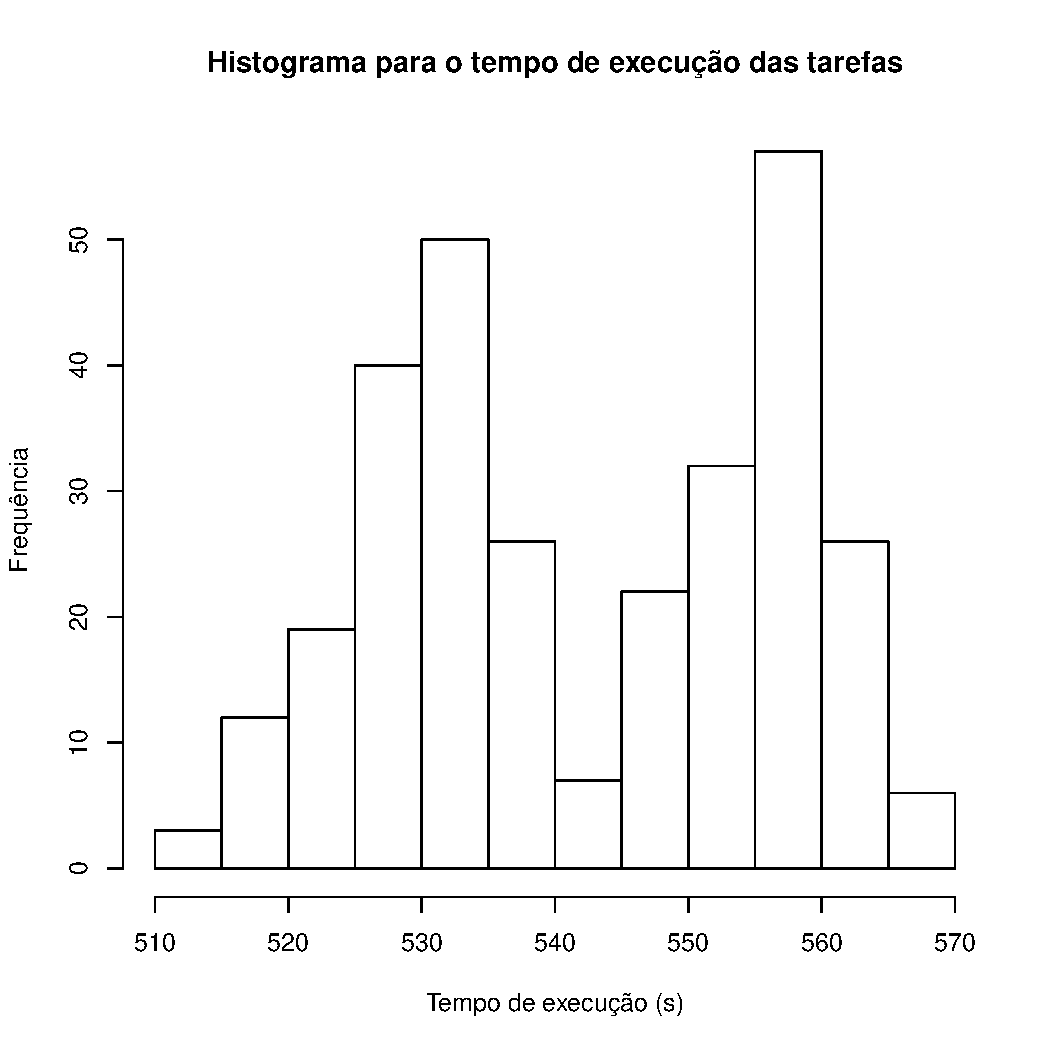
\includegraphics[scale=0.8]{hist_geral.pdf}

	\caption{Histograma dos tempos de execução das tarefas}
	\label{hist_tarefas}
\end{figure}


\begin{figure}[!ht]
	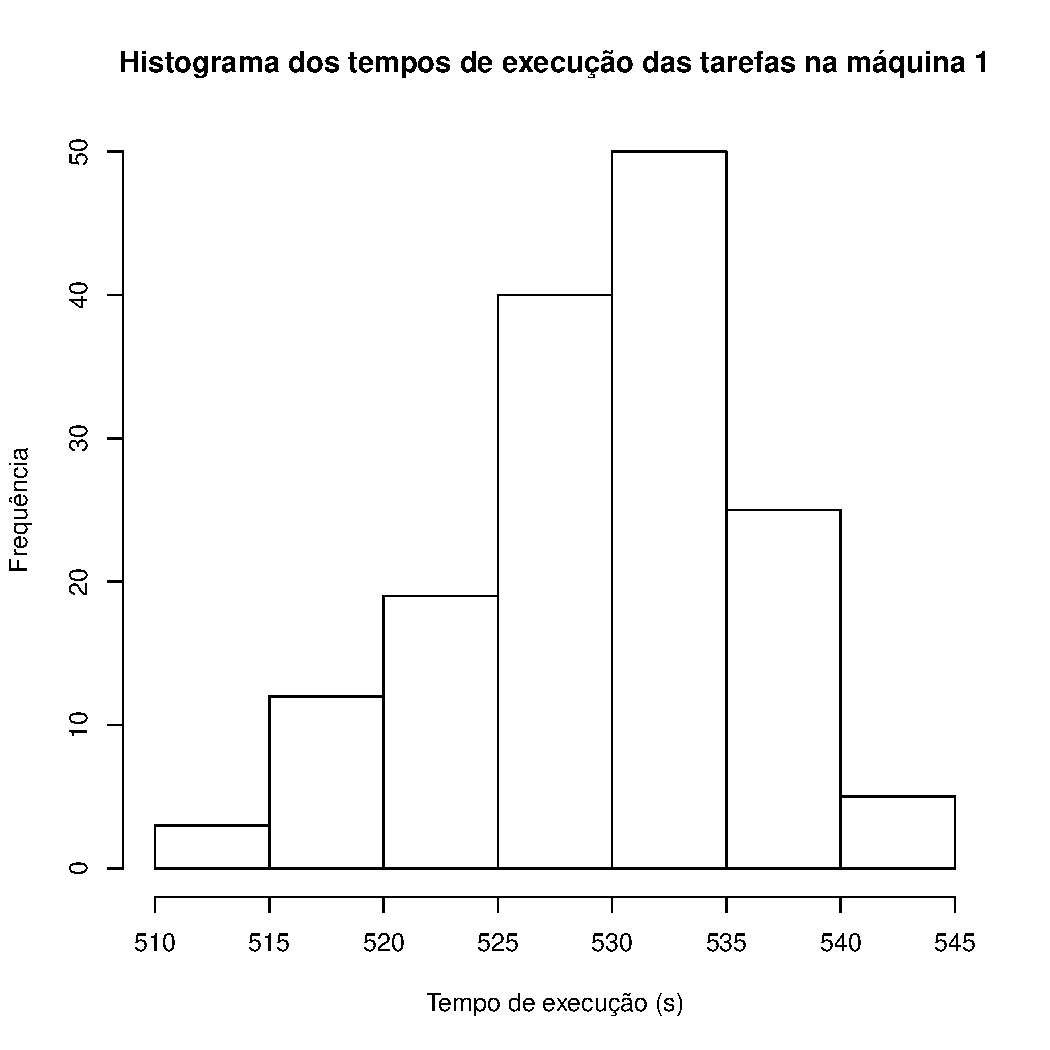
\includegraphics[scale=0.8]{hist1.pdf}

	\caption{Histograma dos tempos de execução das tarefas no computador $1$}
	\label{hist_comp1}
\end{figure}


\begin{figure}[!ht]
	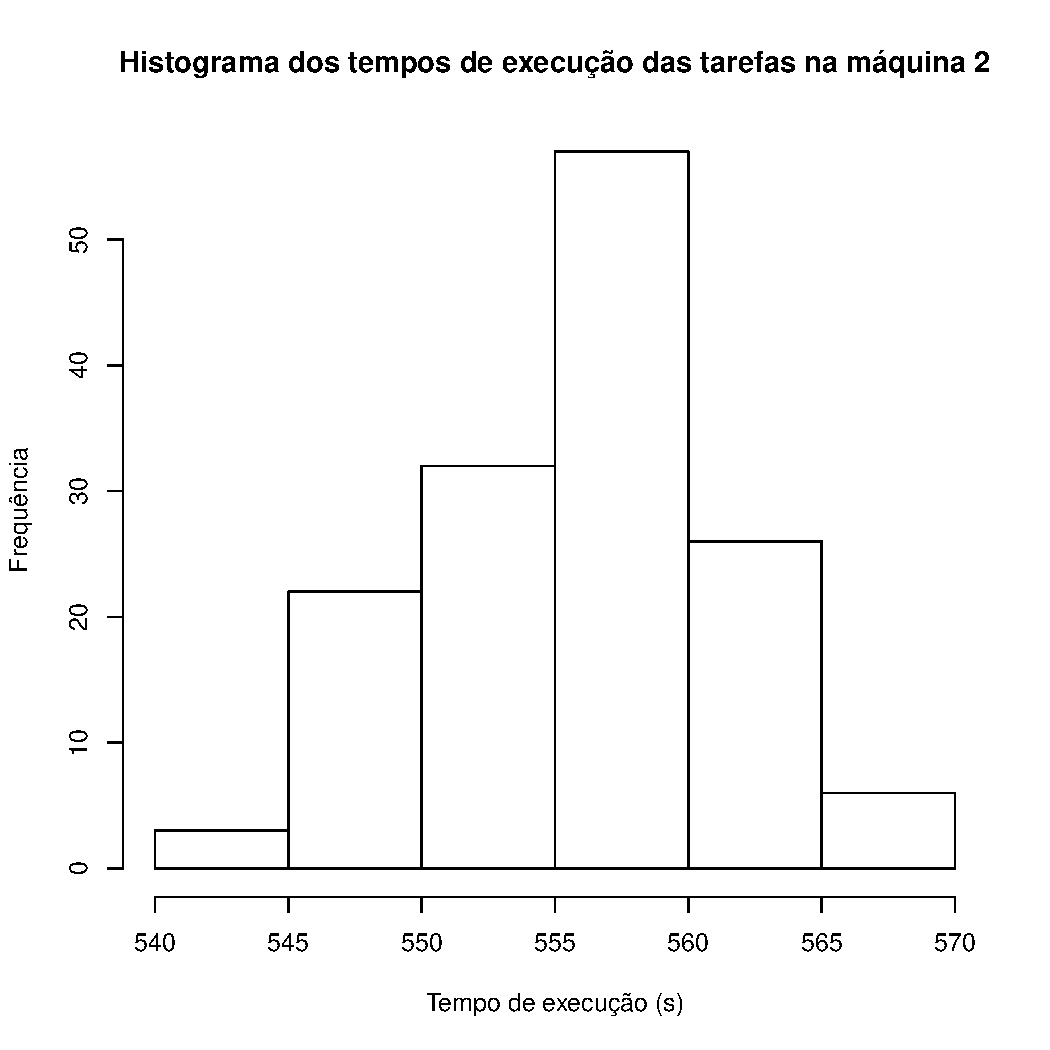
\includegraphics[scale=0.8]{hist2.pdf}

	\caption{Histograma dos tempos de execução das tarefas no computador $2$}
	\label{hist_comp2}	
\end{figure}



O tempo total de processamento das tarefas foi de $14h31min41s$. Caso as tarefas fossem processadas
em série, em um computador e de maneira direta (sem o \emph{BOINC})
o tempo de execução seria de, aproximadamente, $21h40min$ o que nos dá um \emph{speed-up} 
próximo de $1.5$.










\newpage

\section{Conclusões}


A principal conclusão deste trabalho é que é possível a utilização do \emph{BOINC} para o processamento
de rotinas de bioinformática escritas na linguagem \emph{R}. A utilização multiplataforma
também foi de grande utilidade já que podemos incluir praticamente qualquer tipo de computador 
existente em redes. O custo total de implementação foi somente a inutilização de uma máquina, utilizada
como servidor da rede. Embora o \emph{BOINC} seja um projeto consolidado e possua uma documentação com bastante conteúdo,
as mensagens de erro, principalmente do \emph{Wrapper}, são muito pouco informativas, o que tornou o desenvolvimento 
deste projeto bastante trabalhoso. 

A instalação do \emph{BOINC} e do \emph{R} na rede do CEC também foi bastante simples pois estes estão disponíveis
como pacotes do Debian (que é a distribuição Linux que é executada nos laboratórios do CEC). O \emph{deploy} da aplicação
de teste também foi simples, já que o BOINC possui um utilitário de linha de comando e com apenas um comando (apontando 
o servidor e a chave de acesso) o deploy da aplicação é feito.

Para a continuação do projeto há várias sugestões:

\begin{itemize}
  \item \emph{Benchmark} da rede e comparação com grade descrita no artigo \cite{Dias}
Para determinar a viabilidade, seria interessante estabelecermos a comparação com outra 
alternativa. 
  \item Comparação com grades ``alugadas'': hoje já existe oportunidade de se fazer esse tipo de processamento.
em grades alugadas como a oferecida pela empresa \emph{Amazon}. Como os computadores na rede 
consomem energia elétrica seria interessante comparar o gasto da energia elétrica com o gasto em 
uma grade ``alugada''.
  \item Analisar o desempenho nas máquinas com Windows e com Linux. Seria interessante analisar 
o Benchmark da grade em ambos os sistemas e determinar qual das duas plataformas é mais
propícia para o processamento;
  \item Utilização de máquinas virtuais: como feito no artigo \cite{boinc}, podemos utilizar
máquinas virtuais, que são iniciadas em cada nó e é feito o processamento. Sem ter que se preocupar
com a instalação do \emph{R} em todas as máquinas 
\end{itemize}




\newpage

\bibliographystyle{amsalpha}
\bibliography{bibliografia}


\newpage


\part{Parte subjetiva}

Nesta seção descreveremos a relação entre nosso projeto e a experiência adquirida no BCC.

(TODO pensei em fazer separado mas agora que escrevi tenho impressão que não vai mudar muita coisa)

\section{Alberto Ueda}
Entregar este projeto como trabalho de formatura e disponibilizar seu código para os alunos do BCC foram duas das experiências mais gratificantes que já tive. Isto pois acredito que tal conteúdo poderá ser utilizado pelas próximas turmas do BCC como incentivo ao aprendizado da matéria de física. Além disso, tanto alunos do próprio Instituto de Física quanto da Engenharia Politécnica também poderão se interessar pelo conteúdo: o primeiro grupo (FIS) pela animação de fenônemos físicos estudados e o segundo (Poli) tanto pela animação quanto pela simulação de tais fenônemos.

Mas, ao mesmo tempo, por ser um trabalho que levou meses, certas dificuldades foram encontradas pelo caminho. Tivemos que tomar decisões às vezes frustrantes, porém necessárias.

\subsection{Desafios e frustrações encontrados}
Inicialmente, nossa motivação era entregar um sistema que utilize recursos do Wii Remote (TODO ref TODO link da caneta) e que o professor pudesse utilizá-lo em sala de aula para realizar suas simulações e animações. Porém, chegamos a conclusão que esta tecnologia aumentaria consideravelmente o nível de complexidade de nosso trabalho e não tínhamos garantia de que utilizá-la acrescentaria da mesma forma ao resultado final. Assim descartamos esta possibilidade.

Como utilizamos algumas bibliotecas de terceiros em nosso projeto, tivemos que entender obrigatoriamente como eram feitas as principais chamadas de métodos destas bibliotecas, principalmente o Chipmunk e o Gosu. Um detalhe interessante que ocorreu no segundo mês de trabalho foi a necessidade de mudar o código da biblioteca (TOOD citar) e recompilá-la para que uma função simples de mensagem para o usuário funcionasse (TODO conferir método). Uma semana depois, utilizando uma versão mais nova da biblioteca, descobrimos que nossa alteração não era mais necessária, pois já havia sido feita pelos próprios programadores na mudança de versão.

Além disso, utilizamos um binding (TODO envoltório?) da versão original do Chipmunk. Isto trazia duas dificuldades para nós: 1) o código original (em C++) sempre estava com uma versão mais recente e provia (TODO conferir) mais métodos; e 2) nem sempre o que víamos na documentação oficial possuia correspondente em nosso binding. 
 
Por último, um desafio que tivemos foi encontrar um professor de física disponível para nos auxiliar na elaboração do protótipo do sistema. Ficamos muito felizes quando após algumas semanas o bacharel em física e aluno do BCC João Kerr veio a uma de nossas reuniões, a convite do professor Coelho.

\subsection{Disciplinas mais relevantes}

\begin{itemize}

\item MAC0110   Introdução à Computação : Embora já tivesse contato com programação no ensino técnico, foi nesta disciplina que passei a conhecer e utilizar boas práticas de programação. Além disso, estudei algoritmos famosos e interessantes (por exemplo os de ordenação) que estimularam-me para as disciplinas que viriam a seguir.

\item FAP0126 	Física I : É a grande motivação deste trabalho. Os conceitos aprendidos nesta disciplina estão por todo nosso código e nas simulações produzidas. Com o Physimulation, tentamos unir o que vimos nesta disciplina com a computação.
 
\item MAC0122 	Princípios de Desenvolvimento de Algoritmos : O maior contato com algoritmos, dos mais simples e elegantes aos mais complexos, foi fundamental para minha formação. Primeiro porque me desafiou em certos momentos - e consequentemente me deu coragem para analisar ou implementar futuros algoritmos - e em segundo lugar pois deu-me a confiança de que gostaria de seguir carreira em computação.
 
\item MAC0211 	Laboratório de Programação I : Esta disciplina foi interessante por dois motivos: pelo estímulo ao trabalho em equipe e por nos apresentar conceitos e ferramentas relacionadas a qualidade de software, como o Doxygen para documentação de código. Foi nesta disciplina que aprendi o que era um Makefile!

\item MAC0323 	Estruturas de Dados : Essencial para minha formação como cientista da computação. As estruturas aprendidas nesta disciplina - como listas ligadas e árvores - são muito comuns na programação, mesmo no mercado. Possuem vantagens e desvantagens entre si e o conhecimento de suas propriedades assim como os algoritmos adequados para manipulá-las foram muito importantes para mim.

\item MAC0420 	Introdução a Computação Gráfica : Outro forte motivador para nosso trabalho. Nesta disciplina tivemos como exercício-programa a simulação de um jogo de bilhar em três dimensões. Foi uma das experiências mais gratificantes do meu BCC, pois minha dupla e eu aplicamos física em um código simples em C com algumas bibliotecas gráficas e de repente tínhamos uma simulação razoável do que ocorre na vida real. Foi quando percebi que com poucos conceitos de física podíamos reproduzir muitos fenômenos naturais, como colisões e dissipação de energia. Percebi também o quanto estes resultados me motivavam a estudar mais, tanto física quanto computação.

\item FAP0137 	Física II : Os tópicos desta disciplina não foram o foco deste projeto, mas foram grandes motivadores para nosso trabalho. Assim como em Física I, houve pouca contextualização do que foi estudado com o curso de computação. No futuro, temas como relatividade restrita poderão se tornar bem mais simples de se entender por meio de animações criadas pelo próprio usuário, utilizando nosso simulador.
 
\item MAC0332 	Engenharia de Software : na área de computação, um dos conceitos mais recorrentes em qualquer projeto de longo prazo é ciclo de vida de um \textit{software}. Este era o tópico mais discutido na disciplina, tornando-a fundamental para o aluno de computação. Outro aspecto a destacar é a prática de trabalho em equipe.

\item MAC0338 	Análise de Algoritmos: difícil descrever em poucas linhas o quanto esta disciplina é importante para o aluno de computação. Além do desempenho ser uma preocupação constante e necessária a qualquer programador, o aprendizado nesta disciplina é uma das minhas bases sólidas como desenvolvedor. É uma das matérias que quero aprofundar meus conhecimentos durante o mestrado.

\item MAC0446 	Princípios de Interação Homem-computador : uma das disciplinas mais legais para o aluno que está preocupado com a usabilidade de seu sistema. Os conceitos aprendidos estão por todo o trabalho, assim como em outros projetos que participei ou fui responsável.

\end{itemize}
\subsection{Estudos futuros} 
Sem dúvida os tópicos de estudo mais importantes para a continuação deste trabalho são as disciplinas de Física I e II para o BCC. Quanto maior o conhecimento das leis e forças físicas presentes no mundo real, melhor serão as simulações e consequentemente as animações geradas.

Em segundo lugar, seria interessante uma análise de qual das alternativas a seguir tem uma melhor relação custo-benefício, visando a atualização do projeto com a versão mais nova do Chipmunk: A) migrar nosso projeto de Ruby para C++ e usar diretamente a versão original do Chipunk, sem bindings; ou B) atualizar o binding em Ruby adicionando os métodos e funcionalidades da versão mais recente em C++.

Por último, mas não menos importante, um estudo de paradigmas que proporcionem mais usabilidade ao usuário, substituindo o preenchimento obrigatório de formulários para criação de objetos físicos. Ex: \textit{drag-and-drop} do mouse para "arrastar" as formas geométricas, fornecendo os valores de massa, coeficientes de elasticidade e atrito \textit{a posteriori} (após o objeto já estar na tela).


\section{Rafael Miyagawa}



\end{document}
